\documentclass[../main.tex]{subfiles}
\section{Contagion on the Model}

As equation (\ref{local_p_comp}) shows, price contagion depends, via $P(\matr{Y})$, on the matrix $(2\matr{I} + \matr{G})^{-1}$ which we can define as the ``bargaining power'' matrix, since it allocates the excess revenues, $\Delta_t$, among providers in the network. For example, in the case of a positive demand shock and an increase in the local price of electricity of a given node, the excess demand will be partially absorbed by all other nodes in the network which, in turn, causes a contagion of local price hikes. Hence, the spread of the price hikes depends on the bargaining power of nodes in the matrix. Sticking with our example, if $X_{i, t}$ increases suddenly, $\Delta^{(i, j)}_t$ increases, and the cross-border prices across the network increase by
\begin{equation*}
    (2\matr{I} + \matr{G})^{-1}_{(k, l), (i, j)}
\end{equation*}

This implies that a provider with a stronger bargaining position reacts more strongly to price changes, captures higher revenue, which leads to higher prices in the local market. Intuitevely this implies that a denser network, which leads to a more equal distirbution bargaining power, leads to lower revenues for providers and lower price hikes.

\begin{figure}[!ht]
    \centering
    \begin{subfigure}{.5\textwidth}
        \centering
        \includegraphics[width=\textwidth]{\bargpath/line.pdf}
        \caption{On a sequential graph}
        \label{fig:linepower}
    \end{subfigure}%
    \begin{subfigure}{.5\textwidth}
        \centering
        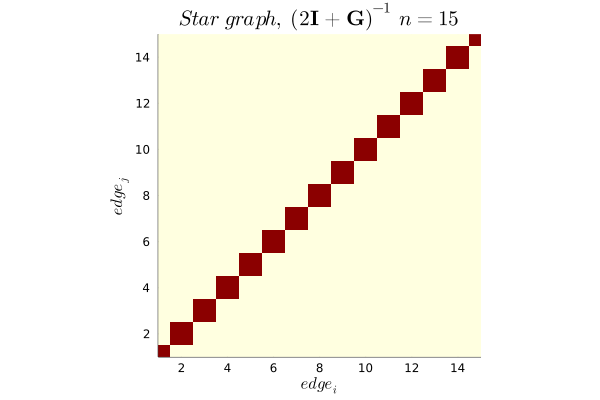
\includegraphics[width=\textwidth]{\bargpath/star.pdf}
        \caption{On a star graph}
        \label{fig:starpower}
    \end{subfigure}
    \caption{Bargaining power, $\sum_{\text{row}} (2\matr{I} + \matr{G})^{-1}$}
\end{figure}


\subsubsection{Contagion simulation}


\begin{figure}[!ht]
    \centering
    \begin{minipage}{.5\textwidth}
        \centering
        \includegraphics[width=\linewidth]{\plotpath/line/pricesupply.pdf}
        \caption{Line}
        \label{fig:lineprice}
    \end{minipage}%
    \begin{minipage}{.5\textwidth}
        \centering
        \includegraphics[width=\linewidth]{\plotpath/smallstar/pricesupply.pdf}
        \caption{Small star}
        \label{fig:smallstarprice}
    \end{minipage}
\end{figure}